\documentclass[12pt, a4paper]{article}


% A pretty common set of packages
\usepackage[margin=2.5cm]{geometry}
\usepackage[T1]{fontenc}
\usepackage{graphicx}
\usepackage{amssymb}
\usepackage{amsmath}
\usepackage{color}
\usepackage{booktabs}
\usepackage{multirow}
\documentclass{memoir}
\usepackage{engord}
\usepackage{enumitem}
\usepackage{soul}
\usepackage{multicol}
\usepackage{textcomp}
\usepackage{parskip}
\usepackage{setspace}
\usepackage{titlesec}
\usepackage{subfig}
\usepackage{float}
\usepackage{adjustbox}
\usepackage[demo]{graphicx}
\usepackage{caption}
\usepackage{subcaption}
\usepackage{siunitx,booktabs,caption}
\usepackage{listings}
\usepackage[spanish]{babel}
\usepackage[skip=2pt,font=footnotesize,justification=centering]{caption}
\usepackage{natbib}
\usepackage[skip=10pt plus1pt, indent=40pt]{parskip}
\usepackage{parskip}
\usepackage[colorlinks=true, 
    linkcolor=blue,          % color of internal links
    citecolor=blue,        % color of links to bibliography
    filecolor=blue,      % color of file links
    urlcolor=blue]{hyperref}



% Do you prefer Sans Serif fonts?
%\usepackage{sfmath}
%\renewcommand{\familydefault}{\sfdefault} 




% Make some additional useful commands
\newcommand{\ie}{\emph{i.e.}\ }
\newcommand{\eg}{\emph{e.g.}\ }
\newcommand{\etal}{\emph{et al}}
\newcommand{\sub}[1]{$_{\textrm{#1}}$}
\newcommand{\super}[1]{$^{\textrm{#1}}$}
\newcommand{\degC}{$^{\circ}$C}
\newcommand{\wig}{$\sim$}
\newcommand{\ord}[1]{\engordnumber{#1}}
\newcommand{\num}[2]{$#1\,$#2}
\newcommand{\range}[3]{$#1$-$#2\,$#3}
\newcommand{\roughly}[2]{$\sim\!#1\,$#2}
\newcommand{\area}[3]{$#1 \! \times \! #2\,$#3}
\newcommand{\vol}[4]{$#1 \! \times \! #2 \! \times \! #3\,$#4}
\newcommand{\cube}[1]{$#1 \! \times \! #1 \! \times \! #1$}
\newcommand{\figref}[1]{Figure~\ref{#1}}
\newcommand{\eqnref}[1]{Equation~\ref{#1}}
\newcommand{\tableref}[1]{Table~\ref{#1}}
\newcommand{\secref}[1]{Section \ref{#1}}
\newcommand{\XC}{\emph{exchange-correlation}}
\newcommand{\abinit}{\emph{ab initio}}
\newcommand{\Abinit}{\emph{Ab initio}}
\newcommand{\Lonetwo}{L1$_{2}$}
\newcommand{\Dznt}{D0$_{19}$}
\newcommand{\Dtf}{D8$_{5}$}
\newcommand{\Btwo}{B$_{2}$}
\newcommand{\fcc}{\emph{fcc}}
\newcommand{\hcp}{\emph{hcp}}
\newcommand{\bcc}{\emph{bcc}}
\newcommand{\Ang}{{\AA}}
\newcommand{\inverseAng}{{\AA}$^{-1}$}
%\newcommand{\comment}[1]{}
\newcommand{\comment}[1]{\textcolor{red}{[COMMENT: #1]}}
\newcommand{\more}{\textcolor{red}{[MORE]}}
\newcommand{\red}[1]{\textcolor{red}{#1}}

\usepackage{capt-of,graphicx}
\newcounter{pics}

\newcommand\z[2][]{%
  \ifnum\value{pics}=4\par\setcounter{pics}{1}\else\stepcounter{pics}\fi
  \ifhmode\unskip\hfill\fi
  \parbox[t]{.50\textwidth}{%
   \centering\includegraphics[width=\linewidth]{#2}\par
   \ifx\relax#1\relax\else\captionof{figure}{#1}\fi}}

\newcommand{\splitcell}[1]{%
  \begin{tabular}{@{}c@{}}\strut#1\strut\end{tabular}%
}

\begin{document}
\thispagestyle{empty}
	
\begin{figure}[ht]
   \minipage{0.76\textwidth}
		
\includegraphics[width=4cm]{fi.png}
		\label{EscudoUABC}
   \endminipage
   \minipage{0.32\textwidth}
		
\includegraphics[height = 4.5 cm ,width=4.5cm]{unam.png}
		\label{EscudoFC}
	\endminipage
\end{figure}
	
\begin{center}
\vspace{0.8cm}
\LARGE
UNIVERSIDAD NACIONAL AUTÓNOMA DE MÉXICO

\vspace{0.8cm}
\LARGE
FACULTAD DE INGENIERÍA

\vspace{1.7cm}	
\Large
\textbf{Proyecto 2}

\vspace{0.2cm}
\LARGE
Analizador Síntactico

\vspace{1.3cm}
\normalsize	
PRESENTA \\
\vspace{.3cm}
\large
\textbf{Navarrete Zamora Aldo Yael}

\vspace{1.3cm}
\normalsize	
PROFESORA \\
\vspace{.3cm}
\large
\textbf{Laura Sandoval Montaño}

\vspace{1.3cm}
\normalsize	
ASIGNATURA \\
\vspace{.3cm}
\large
\textbf{Compiladores}
\end{center}

\newpage

% --- Descripción
\section{Descripción del problema}


\begin{figure}[htpb!]
\centering
  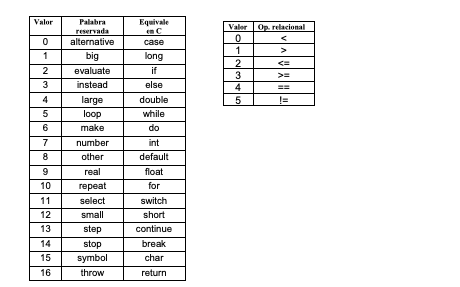
\includegraphics[width=\textwidth]{catalogos.png}
\caption{Catálogos para las palabras reservadas y los operadores relacionales.}
\end{figure}\par


%---- Propuesta de solución
\section{Conjuntos de selección para cada producción}

%----- Ejecución del programa
\section{Ejecución del programa}
El programa se encuentra comentado, con una descripción breve de lo que hace cada una de las funciones. La sangría está muy cuidada y se ve bastante presentable y legible el código.
Para correr el programa, debemos tener instalado flex en nuestro equipo y seguir los siguientes pasos una vez que lo tengamos instalado.

\begin{enumerate}
    \item Abrir en una ventana de terminal la carpeta donde se encuentran todos los archivos.
    \item Una vez dentro de la carpeta correremos el comando \texttt{flex lexical-analyzer.l}
    \item \texttt{gcc lex.yy.c -ly -ll -o lexical-analyzer.out} para compilarlo mediante gcc y tener un archivo de salida ejecutable para un entorno LINUX.
    \item Finalmente, \texttt{./lexical-analyzer.out inputFile.txt} es importante destacar que, el archivo \textit{inputFile.txt} es el archivo de entrada, \textbf{en caso de no teclear ningún archivo de entrada el programa puede manejar este tipo de problema mandando un mensaje de que es necesaria esa entrada por consola.}
\end{enumerate}

Una vez ejecutados los pasos anteriores, podrémos observar \textbf{dos archivos de texto para la salida:}
\begin{enumerate}
    \item El archivo de texto para la generación de los tokens.
    \item El archivo de texto para la la impresión de errores léxicos.
\end{enumerate}

Este último archivo reportará qué expresiones regulares no están definidas por el lenguaje desarrollado.

\section{Conclusiones}
\chapterprecishere{"Hola"}
"\par\raggedleft--- \textup{\textbf{Navarrete Zamora Aldo Yael}}, Estudiante de Ingeniería en Computación}
\end{document}
